\documentclass[border=10pt]{standalone}
\usepackage{pgfplots}
\pgfplotsset{compat=1.17}
\begin{document}
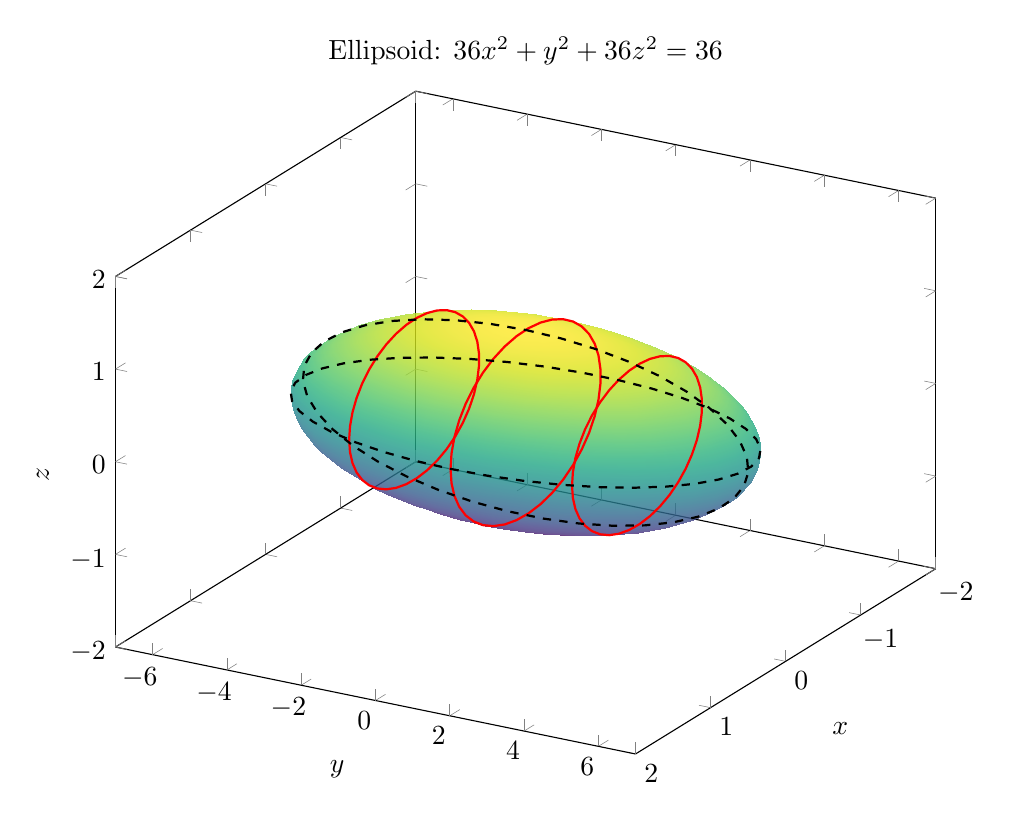
\begin{tikzpicture}
\begin{axis}[
    view={120}{30},
    xlabel=$x$, ylabel=$y$, zlabel=$z$,
    xmin=-2, xmax=2,
    ymin=-7, ymax=7,
    zmin=-2, zmax=2,
    width=12cm, height=10cm,
    samples=40,
    colormap/viridis,
    title={Ellipsoid: $36x^2+y^2+36z^2=36$}
]
\addplot3[
    surf,
    shader=interp,
    opacity=0.8,
    domain=0:180, domain y=0:360,
    z buffer=sort
]
({sin(x)*cos(y)}, {6*sin(x)*sin(y)}, {cos(x)});
% horizontal traces y = k
\addplot3[red, thick, samples y=0, domain=0:360]
({sqrt(1-9/36)*cos(x)}, {3}, {sqrt(1-9/36)*sin(x)});
\addplot3[red, thick, samples y=0, domain=0:360]
({sqrt(1-9/36)*cos(x)}, {-3}, {sqrt(1-9/36)*sin(x)});
\addplot3[red, thick, samples y=0, domain=0:360]
({cos(x)}, {0}, {sin(x)});
% vertical trace z=0
\addplot3[black, dashed, thick, samples y=0, domain=0:360]
({cos(x)}, {6*sin(x)}, {0});
% vertical trace x=0
\addplot3[black, dashed, thick, samples y=0, domain=0:360]
({0}, {6*sin(x)}, {cos(x)});
\end{axis}
\end{tikzpicture}
\end{document}